\documentclass[12pt,a4paper]{article}

%=============================================================================
% PACKAGES
%=============================================================================
\usepackage{amsmath,amssymb,amsthm}
\usepackage{tikz}
\usetikzlibrary{arrows.meta, positioning, calc, decorations.markings}
\usepackage[margin=1in]{geometry}
\usepackage{booktabs}
\usepackage{array}
\usepackage{hyperref}
\usepackage{cleveref}

%=============================================================================
% THEOREM ENVIRONMENTS
%=============================================================================
\newtheorem{theorem}{Theorem}[section]
\newtheorem{proposition}[theorem]{Proposition}
\newtheorem{lemma}[theorem]{Lemma}
\newtheorem{corollary}[theorem]{Corollary}
\newtheorem{definition}[theorem]{Definition}
\newtheorem{remark}[theorem]{Remark}
\newtheorem{example}[theorem]{Example}
\newtheorem{conjecture}[theorem]{Conjecture}

%=============================================================================
% TITLE AND AUTHOR
%=============================================================================
\title{The Hodge--de Rham Complex, Clifford Bundles, and Exceptional Structures:\\
\large From Differential Forms to $E_8$ via Octonionic Geometry}

\author{John A.\ Janik}

\date{\today}

\begin{document}
	
\maketitle

%=============================================================================
% ABSTRACT
%=============================================================================
\begin{abstract}
We present a unified geometric framework connecting the Hodge--de Rham complex on (pseudo-)Riemannian manifolds to Clifford algebra structures and their exceptional extensions. Beginning with the familiar de Rham complex on $\mathbb{R}^3$, we demonstrate how the Hodge star operator, musical isomorphisms, and the exterior derivative organize into a ``diamond'' structure that reveals deep connections between geometry and physics. This structure extends naturally to Minkowski spacetime $\mathbb{R}^{3,1}$, where the self-duality of 2-forms underlies electromagnetic theory and instantons. In seven dimensions, the octonionic structure induces a Hodge--de Rham complex with $G_2$ holonomy, triality symmetry, and connections to M-theory compactifications. The exceptional Jordan algebra $\mathfrak{J}_3(\mathbb{O})$ emerges as the natural coordinate system, with $E_8$ appearing as the internal logic of the extended Hodge--de Rham complex. This framework unifies differential forms, spinors, gauge fields, and gravitational degrees of freedom within a single algebraic structure, suggesting that exceptional geometry is not merely a mathematical curiosity but an essential ingredient for fundamental physics.
\end{abstract}

\tableofcontents
\newpage

%=============================================================================
% SECTION 1: INTRODUCTION
%=============================================================================
\section{Introduction}\label{sec:introduction}

The de Rham complex is one of the foundational structures in differential geometry, encoding the relationship between differential forms of various degrees through the exterior derivative $d$. On a Riemannian or pseudo-Riemannian manifold, the presence of a metric introduces additional structure: the Hodge star operator $\star$, which establishes dualities between forms of complementary degree, and the musical isomorphisms $\flat$ and $\sharp$, which convert between vectors and covectors.

Together, these operators organize the spaces of differential forms into what we call the \textbf{Hodge--de Rham diamond}---a diagrammatic representation that reveals profound connections between geometry and physics. The purpose of this paper is to trace these connections from their simplest manifestation in three-dimensional Euclidean space through progressively richer structures:

\begin{enumerate}
	\item The \textbf{de Rham complex on $\mathbb{R}^3$}, where vector calculus operations (gradient, curl, divergence) are recognized as manifestations of the exterior derivative acting on forms of different degrees.
	
	\item The \textbf{Clifford bundle formalism}, which unifies all differential forms into sections of a single algebraic structure, with the Clifford product encoding both the wedge product and the metric.
	
	\item The \textbf{physical correspondence}, where scalar fields, gauge potentials, field strengths, and currents find their natural home at different levels of the Hodge--de Rham diamond.
	
	\item The \textbf{Minkowski spacetime extension}, where the self-duality of 2-forms gives rise to complex structure, electromagnetic duality, and the mathematical foundation of instantons and twistor theory.
	
	\item The \textbf{octonionic extension in 7 dimensions}, where $G_2$ holonomy, triality, and exceptional structures emerge naturally from the Hodge--de Rham complex.
	
	\item The \textbf{connection to $E_8$}, where the exceptional Jordan algebra $\mathfrak{J}_3(\mathbb{O})$ serves as the coordinate system and $E_8$ appears as the unifying symmetry of the extended structure.
\end{enumerate}

Our central thesis is captured in the following characterization:

\begin{quote}
\textit{$E_8$ is the Lie algebra of the Clifford bundle over an octonionic base, where the Hodge star is extended to a triality operator that unifies differential forms with spinor fields.}
\end{quote}

This treats $E_8$ not as a ``group of matrices'' but as the \textbf{internal logic of the Hodge--de Rham complex itself}.

%=============================================================================
% SECTION 2: THE HODGE--DE RHAM COMPLEX ON R^3
%=============================================================================
\section{The Hodge--de Rham Diamond on $\mathbb{R}^3$}\label{sec:R3}

\subsection{The de Rham Complex}

On a smooth $n$-dimensional manifold $M$, the \textbf{de Rham complex} is the cochain complex
\[
0 \longrightarrow \Omega^0(M) \xrightarrow{d} \Omega^1(M) \xrightarrow{d} \Omega^2(M) \xrightarrow{d} \cdots \xrightarrow{d} \Omega^n(M) \longrightarrow 0,
\]
where $\Omega^k(M)$ denotes the space of smooth $k$-forms and $d$ is the exterior derivative satisfying $d^2 = 0$.

For $\mathbb{R}^3$ with coordinates $(x,y,z)$, the spaces are:
\begin{align*}
\Omega^0 &= \{f(x,y,z)\} & &\text{(scalar fields)} \\
\Omega^1 &= \{f_x\,dx + f_y\,dy + f_z\,dz\} & &\text{(1-forms)} \\
\Omega^2 &= \{g_x\,dy \wedge dz + g_y\,dz \wedge dx + g_z\,dx \wedge dy\} & &\text{(2-forms)} \\
\Omega^3 &= \{h\,dx \wedge dy \wedge dz\} & &\text{(3-forms/top forms)}
\end{align*}

\subsection{The Hodge Star Operator}

On an oriented Riemannian $n$-manifold $(M,g)$, the \textbf{Hodge star} is the linear isomorphism
\[
\star: \Omega^k(M) \xrightarrow{\cong} \Omega^{n-k}(M)
\]
defined by the condition $\alpha \wedge \star\beta = g(\alpha,\beta)\,\mathrm{vol}_g$ for all $k$-forms $\alpha,\beta$.

On $\mathbb{R}^3$ with the Euclidean metric:
\begin{align*}
\star 1 &= dx \wedge dy \wedge dz, & \star(dx \wedge dy \wedge dz) &= 1, \\
\star dx &= dy \wedge dz, & \star(dy \wedge dz) &= dx, \\
\star dy &= dz \wedge dx, & \star(dz \wedge dx) &= dy, \\
\star dz &= dx \wedge dy, & \star(dx \wedge dy) &= dz.
\end{align*}

In dimension $n$ with signature $(p,q)$, we have $\star^2 = (-1)^{k(n-k)+q}$ on $k$-forms.

\subsection{The Codifferential and Hodge--Laplacian}

The \textbf{codifferential} is defined as
\[
\delta = (-1)^{n(k+1)+1}\star d\star: \Omega^k \to \Omega^{k-1},
\]
satisfying $\delta^2 = 0$. The \textbf{Hodge--Laplacian} is
\[
\Delta = d\delta + \delta d = (d + \delta)^2.
\]

\subsection{Musical Isomorphisms}

Given a metric $g$, the \textbf{flat} and \textbf{sharp} maps convert between vectors and 1-forms:
\begin{align*}
\flat: \Gamma(TM) &\to \Omega^1(M), & X &\mapsto g(X,\cdot), \\
\sharp: \Omega^1(M) &\to \Gamma(TM), & \omega &\mapsto g^{-1}(\omega,\cdot).
\end{align*}

\subsection{The Diamond Diagram}

The following diagram encodes the full structure of the Hodge--de Rham complex on $\mathbb{R}^3$:

\begin{center}
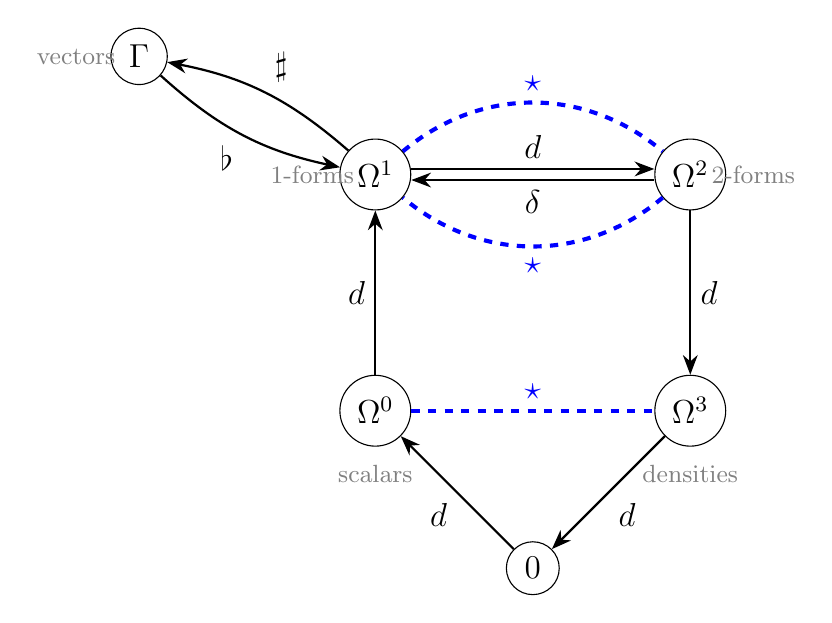
\begin{tikzpicture}[
    node distance=2.5cm and 3cm,
    every node/.style={font=\large},
    arrow/.style={-{Stealth[length=2.5mm]}, thick},
    hodge/.style={blue, dashed, line width=1.5pt},
    parallel shift/.style={transform canvas={yshift=#1}}
]

% === NODES ===
\node [draw, circle] (zero) at (0,-3.5) {$0$};
\node [draw, circle] (omega0) at (-2, -1.5) {$\Omega^0$};
\node [draw, circle] (omega3) at (2, -1.5) {$\Omega^3$};
\node [draw, circle] (omega1) at (-2, 1.5) {$\Omega^1$};
\node [draw, circle] (omega2) at (2, 1.5) {$\Omega^2$};
\node [draw, circle] (Gamma) at (-5, 3) {$\Gamma$};

% === DE RHAM COMPLEX ARROWS (d) ===
\draw[arrow] (zero) -- node[midway, below left] {$d$} (omega0);
\draw[arrow] (omega0) -- node[midway, left] {$d$} (omega1);
\draw[arrow, parallel shift=2pt] (omega1) -- node[midway, above] {$d$} (omega2);
\draw[arrow, parallel shift=-2pt] (omega2) -- node[midway, below] {$\delta$} (omega1);
\draw[arrow] (omega2) -- node[midway, right] {$d$} (omega3);
\draw[arrow] (omega3) -- node[midway, below right] {$d$} (zero);

% === HODGE STAR ARROWS (★) ===
\draw[hodge] (omega0) -- node[midway, above] {$\star$} (omega3);
\draw[hodge, bend left=40] (omega1) to node[midway, above] {$\star$} (omega2);
\draw[hodge, bend left=40] (omega2) to node[midway, below] {$\star$} (omega1);

% === MUSICAL ISOMORPHISMS (♭ and ♯) ===
\draw[-{Stealth[length=2.5mm]}, thick, bend right=15] 
    (Gamma) to node[midway, below left] {$\flat$} (omega1);
\draw[-{Stealth[length=2.5mm]}, thick, bend right=15] 
    (omega1) to node[midway, above right] {$\sharp$} (Gamma);

% === LABELS ===
\node[text=gray, font=\small] at (-2, -2.3) {scalars};
\node[text=gray, font=\small] at (2, -2.3) {densities};
\node[text=gray, font=\small] at (-2.8, 1.5) {1-forms};
\node[text=gray, font=\small] at (2.8, 1.5) {2-forms};
\node[text=gray, font=\small] at (-5.8, 3) {vectors};

\end{tikzpicture}
\end{center}

\noindent\textbf{Key:}
\begin{itemize}
\item $d$ = exterior derivative (raises degree)
\item $\delta = \star d \star$ = codifferential (lowers degree)  
\item $\star$ = Hodge star (duality between complementary degrees)
\item $\flat/\sharp$ = musical isomorphisms (metric-dependent)
\end{itemize}

\subsection{Vector Calculus in Disguise}

The de Rham complex on $\mathbb{R}^3$, when translated through the metric isomorphisms, becomes the familiar sequence of vector calculus:
\[
0 \longrightarrow C^\infty(\mathbb{R}^3) \xrightarrow{\nabla} \mathfrak{X}(\mathbb{R}^3) \xrightarrow{\nabla\times} \mathfrak{X}(\mathbb{R}^3) \xrightarrow{\nabla\cdot} C^\infty(\mathbb{R}^3) \longrightarrow 0.
\]

The correspondence is:
\begin{center}
\renewcommand{\arraystretch}{1.3}
\begin{tabular}{@{}ccccc@{}}
\toprule
\textbf{Forms} & $\Omega^0 \xrightarrow{d} \Omega^1$ & $\Omega^1 \xrightarrow{d} \Omega^2$ & $\Omega^2 \xrightarrow{d} \Omega^3$ \\
\midrule
\textbf{Vector calculus} & $\mathrm{grad}$ & $\mathrm{curl}$ & $\mathrm{div}$ \\
\textbf{Isomorphism} & $\sharp$ & $\star\sharp$ & $\star$ \\
\bottomrule
\end{tabular}
\end{center}

The identities $\mathrm{curl} \circ \mathrm{grad} = 0$ and $\mathrm{div} \circ \mathrm{curl} = 0$ are simply the statement $d^2 = 0$.

%=============================================================================
% SECTION 3: THE CLIFFORD BUNDLE
%=============================================================================
\section{The Clifford Bundle Formalism}\label{sec:clifford}

\subsection{Definition of the Clifford Bundle}

\begin{definition}[Clifford Bundle]
Let $(M,g)$ be a (pseudo-)Riemannian manifold. The \textbf{Clifford bundle} $\mathcal{C}\ell(M,g)$ is the vector bundle whose fiber at each point $x \in M$ is the Clifford algebra $\mathcal{C}\ell(T_xM, g_x)$:
\[
\mathcal{C}\ell(M,g) = \frac{\bigoplus_{k=0}^{\infty} T^{(k)}M}{\langle v \otimes v - g(v,v) \cdot 1 \rangle}
\]
where the ideal imposes the \textbf{Clifford relation} $v \cdot v = g(v,v)$.
\end{definition}

A section $\psi \in \Gamma(\mathcal{C}\ell(M,g))$ expands locally as:
\[
\psi(x) = f(x) + v^i(x)e_i + \tfrac{1}{2!}F^{ij}(x)e_i \wedge e_j + \tfrac{1}{3!}T^{ijk}(x)e_i \wedge e_j \wedge e_k + \cdots
\]
where $\{e_i\}$ is a local orthonormal frame for $TM$ and the coefficients are smooth functions.

\subsection{Physical Correspondence by Grade}

Sections of $\mathcal{C}\ell(M,g)$ are \textbf{multivector fields}, unifying different geometric and physical objects:

\begin{center}
\renewcommand{\arraystretch}{1.4}
\begin{tabular}{c >{\raggedright}p{3.5cm} p{8.5cm}}
\toprule
\textbf{Grade} & \textbf{Mathematical Object} & \textbf{Physical Examples} \\
\midrule
0 & Scalar field & Higgs field $\phi$, dilaton, cosmological constant $\Lambda$, wave function amplitude \\
1 & Vector field / 1-form & 4-potential $A_\mu$, momentum $p_\mu$, current density $j^\mu$, velocity field \\
2 & Bivector / 2-form & Electromagnetic field $F_{\mu\nu}$, angular momentum $L_{\mu\nu}$, Riemann curvature \\
3 & Trivector / 3-form & Torsion $T_{\mu\nu\rho}$, M-theory C-field $C_{\mu\nu\rho}$, Hodge dual of current \\
4 & Pseudoscalar / 4-form & Volume form $\epsilon_{\mu\nu\rho\sigma}$, axion field, $\theta$-term in QCD, chirality operator $\gamma^5$ \\
\bottomrule
\end{tabular}
\end{center}

\subsection{Unified Operators and Field Equations}

The Clifford bundle formalism allows fundamental field equations to be written in remarkably unified forms.

\subsubsection{The Dirac--de Rham Operator}

The \textbf{geometric derivative} $D = d + \delta$ unifies the exterior derivative and codifferential:
\[
D^2 = (d + \delta)^2 = d\delta + \delta d = \Delta \qquad \text{(Hodge--Laplacian)}
\]

\subsubsection{Maxwell's Equations}

In the Clifford formalism, Maxwell's four equations collapse to one:
\[
\boxed{\nabla F = J}
\]
where $F = \mathbf{E} + I\mathbf{B} \in \Gamma(\mathcal{C}\ell(M,g))$ is a bivector field, $J = \rho - \mathbf{j}$ is a vector field, $\nabla = \gamma^\mu \partial_\mu$ is the vector derivative, and $I$ is the pseudoscalar unit.

\subsubsection{The Dirac Equation}

The Dirac equation in Clifford form:
\[
\nabla \psi I \sigma_3 - eA \psi = m \psi \gamma_0
\]
where $\psi \in \Gamma(\mathcal{C}\ell(M,g))$ is an even multivector representing the Dirac spinor.

\subsubsection{Einstein Field Equations}

In the gravitational gauge theory approach:
\[
\mathcal{G}(a) = 8\pi T(a)
\]
where $\mathcal{G}(a)$ is the Einstein tensor as a vector-valued function and $T(a)$ is the stress-energy tensor.

\subsection{Advantages of the Clifford Bundle Formalism}

\begin{enumerate}
\item \textbf{Coordinate Independence}: Physical laws are manifestly coordinate-free and geometric.

\item \textbf{Unification of Algebra and Geometry}: The Clifford product combines wedge (geometry) and inner (metric) products.

\item \textbf{Spinors as Minimal Ideals}: Spinor fields emerge naturally as minimal left ideals of the Clifford algebra.

\item \textbf{Computational Efficiency}: Often simplifies calculations in relativistic physics and general relativity.

\item \textbf{Quantum--Classical Bridge}: The same framework describes classical fields (multivectors) and quantum fields (spinor representations).
\end{enumerate}

%=============================================================================
% SECTION 4: THE CENTRALITY OF Ω²
%=============================================================================
\section{The Centrality of $\Omega^2$: The Dynamics Level}\label{sec:omega2}

\subsection{Why 2-Forms Are Central}

Placing $\Omega^2$ at the geometric center of the diagram reveals deep physical significance.

\subsubsection{Field Strength Lives in $\Omega^2$}

In gauge theory, the hierarchy is:
\[
\underbrace{\Omega^0}_{\text{gauge function}} \xrightarrow{d} 
\underbrace{\Omega^1}_{\text{potential } A} \xrightarrow{d} 
\underbrace{\Omega^2}_{\text{field strength } F} \xrightarrow{d} 
\underbrace{\Omega^3}_{\text{Bianchi } dF=0}
\]

The physics (energy, equations of motion, observables) lives at $\Omega^2$:
\begin{itemize}
\item Electromagnetic field: $F = dA \in \Omega^2$
\item Yang--Mills curvature: $F = dA + A \wedge A \in \Omega^2$
\item Riemann curvature: $R^a{}_b \in \Omega^2(\mathfrak{so}(n))$
\end{itemize}

\subsubsection{$\Omega^2$ Is the Self-Dual Level (in 4D)}

In 4 dimensions, the Hodge star satisfies $\star: \Omega^2 \to \Omega^2$ with $\star^2 = +1$ (Euclidean) or $\star^2 = -1$ (Lorentzian). This allows decomposition into self-dual and anti-self-dual parts:
\[
\Omega^2 = \Omega^2_+ \oplus \Omega^2_-
\]
This is central to instantons, twistor theory, chiral structure of spinors, and Donaldson theory.

\subsubsection{Symplectic Structure}

In Hamiltonian mechanics, the symplectic form $\omega \in \Omega^2(T^*M)$:
\[
\omega = dp_i \wedge dq^i
\]
Phase space geometry is fundamentally $\Omega^2$-geometry.

\subsubsection{The Flux Interpretation}

\begin{center}
\begin{tabular}{c|c|c}
\textbf{Form} & \textbf{Integrates over} & \textbf{Physical meaning} \\
\hline
$\Omega^0$ & point & field value \\
$\Omega^1$ & curve & work, circulation \\
$\Omega^2$ & surface & \textbf{flux} \\
$\Omega^3$ & volume & total charge/mass
\end{tabular}
\end{center}

Flux through surfaces is the natural ``middle'' concept connecting local (differential) to global (integral) physics.

\begin{remark}[Emergent Complex Structure]
The Hodge star $\star$ acts as a complex structure ($J$) on $\Omega^2$ in Minkowski space because $\star^2 = -1$ on 2-forms. This explains why complex numbers appear naturally in physics---they are an emergent property of the geometry of 2-forms.
\end{remark}

%=============================================================================
% SECTION 5: MINKOWSKI SPACE
%=============================================================================
\section{The Hodge--de Rham Complex in Minkowski Space}\label{sec:minkowski}

\subsection{The Extended Diamond in 4D}

For Minkowski space $\mathbb{R}^{3,1}$ with signature $(+,+,+,-)$, the de Rham complex extends to:
\[
0 \to \Omega^0 \xrightarrow{d} \Omega^1 \xrightarrow{d} \Omega^2 \xrightarrow{d} \Omega^3 \xrightarrow{d} \Omega^4 \to 0
\]

The Hodge star satisfies $\star^2 = (-1)^{k(4-k)+1}$ on $k$-forms:
\begin{itemize}
\item $\Omega^0 \xleftrightarrow{\star} \Omega^4$: $\star^2 = -1$
\item $\Omega^1 \xleftrightarrow{\star} \Omega^3$: $\star^2 = +1$
\item $\Omega^2 \xrightarrow{\star} \Omega^2$: $\star^2 = -1$ (complex structure)
\end{itemize}

\subsection{Physical Interpretation of Form Degrees}

\begin{enumerate}
\item \textbf{$\Omega^0$: Scalar Fields} --- Higgs field, dilaton, conformal factors

\item \textbf{$\Omega^1$: 4-Potentials} --- Electromagnetic potential $A = A_\mu dx^\mu$, connection 1-forms, gravitational tetrad $e^a = e^a_\mu dx^\mu$

\item \textbf{$\Omega^2$: Field Strengths} --- Electromagnetic field $F = dA$, Yang--Mills curvature $F = dA + A \wedge A$, Riemann curvature 2-form

\item \textbf{$\Omega^3$: Currents and Sources} --- Electromagnetic current 3-form $J = \star j$, stress-energy currents

\item \textbf{$\Omega^4$: Lagrangians and Topological Terms} --- Volume form, Lagrangian densities $\mathcal{L}\,\mathrm{vol}_4$, Pontryagin density
\end{enumerate}

\subsection{Self-Duality and Instantons}

Since $\star^2 = -1$ on 2-forms, we define complex self-dual and anti-self-dual parts:
\[
F_{\pm} = \frac{1}{2}(F \mp i\star F), \qquad \star F_{\pm} = \pm i F_{\pm}.
\]
This decomposition is fundamental to:
\begin{itemize}
\item Instantons in Yang--Mills theory ($F = \star F$ becomes $F_- = 0$)
\item Twistor theory and the Penrose transform
\item Chiral representations of the Lorentz group
\item Maxwell's equations in vacuum: $dF = 0$ and $d\star F = 0$ imply $dF_{\pm} = 0$
\end{itemize}

%=============================================================================
% SECTION 6: THE OCTONIONIC EXTENSION
%=============================================================================
\section{The Octonionic Hodge--de Rham Complex}\label{sec:octonionic}

\subsection{The Special Status of 7 Dimensions}

The Hodge--de Rham complex for the Clifford algebra $\mathrm{Cl}(0,7)$ represents one of the most physically rich structures in modern theoretical physics. Seven dimensions hold a privileged position because of the connection to octonions and $G_2$ holonomy.

\subsubsection{$G_2$ as the Smallest Exceptional Lie Group}

The exceptional Lie group $G_2 \subset \mathrm{SO}(7)$ with $\dim(G_2) = 14$ preserves the octonionic structure and decomposes the form spaces:
\begin{align*}
\Omega^1(\mathbb{R}^7) &= \Lambda^1_7 &&\text{(fundamental representation)} \\
\Omega^2(\mathbb{R}^7) &= \Lambda^2_7 \oplus \Lambda^2_{14} &&\text{where } \Lambda^2_{14} \cong \mathfrak{g}_2 \\
\Omega^3(\mathbb{R}^7) &= \Lambda^3_1 \oplus \Lambda^3_7 \oplus \Lambda^3_{27}
\end{align*}

\subsection{The Associative and Coassociative Forms}

\subsubsection{The Associative 3-Form $\varphi$}

Defined by octonion multiplication:
\[
\varphi_{ijk} = \langle e_i \times_{\mathbb{O}} e_j, e_k \rangle
\]
This form encodes:
\begin{itemize}
\item $G_2$ structure on 7-manifolds
\item Calibrations for minimal submanifolds
\item Torsion-free condition: $d\varphi = 0$ and $d\star\varphi = 0$ defines $G_2$ holonomy
\end{itemize}

\subsubsection{The Coassociative 4-Form $\star\varphi$}

The Hodge dual satisfies the remarkable relation:
\[
\star\varphi = \frac{1}{2}\varphi \wedge \varphi
\]
This is crucial for topological field theory on $G_2$ manifolds, Donaldson--Thomas invariants, and M-theory.

\subsection{Octonionic Triality}

The triality of $\mathrm{Spin}(8)$:
\[
8_v \otimes 8_s \otimes 8_c \quad \text{with symmetry group } S_3
\]
where $8_v$, $8_s$, $8_c$ are vector, spinor, and conjugate spinor representations.

Physical manifestations include:
\begin{itemize}
\item Superstring theory dualities (Type IIA, IIB, heterotic)
\item U-duality in toroidal compactifications
\item Possible connection to three generations of fermions
\end{itemize}

\subsection{Applications to M-Theory}

\subsubsection{M-Theory Compactifications}

Compactification of 11-dimensional supergravity on 7D $G_2$ holonomy manifolds preserves $\mathcal{N}=1$ supersymmetry in 4D:
\[
\text{M-theory on } \mathbb{R}^{1,3} \times X_{G_2} \to \mathcal{N}=1 \text{ supergravity in 4D}
\]

\subsubsection{Superpotential from the Associative 3-Form}

The associative 3-form $\varphi \in \Omega^3_1$ generates the superpotential:
\[
W = \int_{X_{G_2}} C \wedge \varphi
\]
where $C$ is the M-theory 3-form field.

\subsubsection{Calibrated Cycles and Branes}

Associative 3-cycles are natural worldvolumes for M2-branes, while coassociative 4-cycles support M5-branes.

%=============================================================================
% SECTION 7: THE EXCEPTIONAL JORDAN ALGEBRA
%=============================================================================
\section{The Exceptional Jordan Algebra and $E_8$}\label{sec:jordan}

\subsection{The Albert Algebra}

\begin{definition}[Albert Algebra]
The \textbf{exceptional Jordan algebra} $\mathfrak{J}_3(\mathbb{O})$ is the algebra of $3 \times 3$ Hermitian matrices over the octonions:
\[
\mathfrak{J}_3(\mathbb{O}) = \left\{ 
\begin{pmatrix}
a & x & \bar{y} \\
\bar{x} & b & z \\
y & \bar{z} & c
\end{pmatrix} : a,b,c \in \mathbb{R}, \; x,y,z \in \mathbb{O}
\right\}
\]
with Jordan product $X \circ Y = \frac{1}{2}(XY + YX)$.
\end{definition}

This 27-dimensional algebra possesses extraordinary properties:
\begin{itemize}
\item \textbf{Non-associative but power-associative}: $(A \circ B) \circ A^2 = A \circ (B \circ A^2)$
\item \textbf{Exceptional}: Cannot be realized as a subalgebra of an associative algebra
\item \textbf{Symmetry group}: Automorphism group is the exceptional Lie group $F_4$
\end{itemize}

\subsection{Jordan Algebra $\leftrightarrow$ Form Decomposition}

The decomposition of differential forms under $G_2$ corresponds to the structure of $\mathfrak{J}_3(\mathbb{O})$:

\begin{center}
\begin{tabular}{c|c|c}
\textbf{Form Space} & \textbf{$G_2$ Decomposition} & \textbf{Jordan Component} \\
\hline
$\Omega^0$ & $\mathbb{R}$ & Trace: $\mathrm{tr}(J)$ \\
$\Omega^1$ & $\Lambda^1_7$ & Off-diagonal octonions \\
$\Omega^2$ & $\Lambda^2_7 \oplus \Lambda^2_{14}$ & Jordan multiplication \\
$\Omega^3$ & $\Lambda^3_1 \oplus \Lambda^3_7 \oplus \Lambda^3_{27}$ & $\Lambda^3_{27} \cong \mathfrak{J}_3(\mathbb{O})_0$ \\
\end{tabular}
\end{center}

The key isomorphism is:
\[
\Lambda^3_{27} \cong \mathfrak{J}_3(\mathbb{O})_0 \quad \text{(27-dimensional traceless Jordan matrices)}
\]

\subsection{The Freudenthal--Tits Magic Square}

The exceptional Lie groups form the ``magic square'' via Jordan algebras:
\[
\begin{array}{c|cccc}
& \mathbb{R} & \mathbb{C} & \mathbb{H} & \mathbb{O} \\
\hline
\mathbb{R} & \mathrm{SO}(3) & \mathrm{SU}(3) & \mathrm{Sp}(3) & F_4 \\
\mathbb{C} & \mathrm{SU}(3) & \mathrm{SU}(3)^2 & \mathrm{SU}(6) & E_6 \\
\mathbb{H} & \mathrm{Sp}(3) & \mathrm{SU}(6) & \mathrm{SO}(12) & E_7 \\
\mathbb{O} & F_4 & E_6 & E_7 & E_8
\end{array}
\]

\subsection{The $E_8$ Decomposition}

The 248-dimensional adjoint representation of $E_8$ decomposes as:
\[
\mathbf{248} = \underbrace{\mathbf{120}}_{\mathrm{Adj}(\mathrm{SO}(16))} \oplus \underbrace{\mathbf{128}}_{\mathrm{Spinor}(\mathrm{SO}(16))}
\]

\begin{itemize}
\item \textbf{The 120 (Forms)}: Bivectors/2-forms $\Omega^2$ of a 16-dimensional space---the ``Dynamics'' level.
\item \textbf{The 128 (Spinors)}: Sections of the Spinor Bundle---``Matter'' fields.
\end{itemize}

\textbf{Unified Interpretation}: $E_8$ is the algebra where 2-forms and spinors are rotated into one another. The distinction between ``force'' (form) and ``matter'' (spinor) is merely a choice of perspective within the $E_8$ frame.

\subsection{$E_8$ and the Albert Algebra}

The exceptional Jordan algebra serves as the ``coordinate system'' for $E_8$:
\[
\mathfrak{e}_8 \approx \mathrm{Der}(\mathfrak{J}_3(\mathbb{O})) \oplus \mathfrak{J}_3(\mathbb{O}) \oplus \cdots
\]
$E_8$ is the sum of the symmetries of the diamond plus the nodes of the diamond.

\subsection{Jordan Algebraic Operations in the Hodge--de Rham Complex}

\subsubsection{Metric from Jordan Trace Form}

The inner product on forms can be expressed via Jordan trace:
\[
\langle \omega, \eta \rangle = \mathrm{Tr}(J_\omega \circ J_\eta)
\]

\subsubsection{Associative 3-Form as Jordan Determinant}

The associative 3-form $\varphi$ corresponds to the Jordan determinant:
\[
\det(J) = \frac{1}{3}\mathrm{Tr}(J^3) - \frac{1}{2}\mathrm{Tr}(J^2)\mathrm{Tr}(J) + \frac{1}{6}\mathrm{Tr}(J)^3
\]

\subsubsection{Exterior Derivative as Jordan Derivation}

The exterior derivative $d$ corresponds to Jordan derivations:
\[
D_X(Y) = X \circ Y - Y \circ X
\]
The condition $d^2 = 0$ translates to:
\[
D_X D_Y + D_Y D_X = D_{X \circ Y}
\]

%=============================================================================
% SECTION 8: PHYSICAL IMPLICATIONS
%=============================================================================
\section{Physical Implications}\label{sec:physics}

\subsection{Connections to Particle Physics}

\subsubsection{Exceptional Grand Unification}

The exceptional Lie group $E_6$ contains $G_2$ and provides a natural grand unified theory:
\[
E_6 \supset \mathrm{SO}(10) \times \mathrm{U}(1) \supset \mathrm{SU}(5) \times \mathrm{U}(1)^2
\]
Octonionic structures may explain three generations of fermions, Yukawa couplings, and CKM matrix structure.

\subsubsection{Higher Gauge Theory}

The forms correspond to higher gauge fields:
\begin{align*}
\Omega^1 &: \text{Connection 1-forms} \\
\Omega^2 &: \text{Curvature 2-forms} \\
\Omega^3 &: \text{2-gerbe connections (M-theory C-field)} \\
\Omega^4 &: \text{Field strengths for 3-form gauge fields}
\end{align*}

\subsection{Black Hole Entropy and Jordan Algebras}

The 27-dimensional $\mathfrak{J}_3(\mathbb{O})$ appears in M-theory compactifications:
\begin{itemize}
\item Black hole charges in 5D are described by Jordan algebra elements
\item Entropy formula: $S = \pi \sqrt{\det(J)}$ where $J \in \mathfrak{J}_3(\mathbb{O})$
\item U-duality: The $E_6$ symmetry acts on the 27 charges
\end{itemize}

\subsection{Quantum Information and $G_2$ Codes}

The octonionic Hodge--de Rham complex resembles quantum computational structures:
\begin{itemize}
\item 7-qubit error correction via $G_2$ codes
\item Non-associative generalization of quantum theory
\item Topological quantum computing with $G_2$ manifolds
\end{itemize}

%=============================================================================
% SECTION 9: CONCLUSIONS
%=============================================================================
\section{Conclusions}\label{sec:conclusions}

The Hodge--de Rham complex, when enriched with the Clifford bundle structure and extended to exceptional geometries, provides a unified framework connecting:

\begin{enumerate}
\item \textbf{Differential Geometry}: Exterior calculus, Hodge theory, de Rham cohomology

\item \textbf{Clifford Algebra}: Unified treatment of tensors and spinors, geometric calculus

\item \textbf{Gauge Theory}: Connections, curvature, field equations as manifestations of $d$ and $\delta$

\item \textbf{Exceptional Geometry}: $G_2$ holonomy, octonions, triality

\item \textbf{String/M-Theory}: Compactifications, dualities, branes

\item \textbf{Jordan Algebras}: The Albert algebra as coordinate system for exceptional structures
\end{enumerate}

The central insight is that the \textbf{Hodge--de Rham diamond is not merely a diagram but the organizational principle of physical reality}. Each node represents a sector of the theory, each arrow a physical transformation or duality, and the overall structure encodes the symmetries and dynamics of a unified theory.

The exceptional structures ($G_2$, $F_4$, $E_6$, $E_7$, $E_8$) are not accidental mathematical artifacts but essential ingredients for fundamental physics. The octonionic Hodge--de Rham complex shows precisely how these elements fit together in a coherent, geometrically natural framework.

\begin{center}
\fbox{\parbox{0.9\textwidth}{\centering\itshape
``$E_8$ is the Lie Algebra of the Clifford Bundle over an Octonionic base, where the Hodge Star is extended to a Triality operator that unifies differential forms with spinor fields.''
}}
\end{center}

This treats $E_8$ not as a group of matrices, but as the internal logic of the Hodge--de Rham complex itself.

%=============================================================================
% ACKNOWLEDGMENTS
%=============================================================================
\section*{Acknowledgments}

[Acknowledgments to be added]

%=============================================================================
% BIBLIOGRAPHY
%=============================================================================
\begin{thebibliography}{99}

\bibitem{Baez2002}
J.~C.~Baez, ``The octonions,'' \textit{Bull.\ Amer.\ Math.\ Soc.} \textbf{39} (2002), 145--205.

\bibitem{BrauerRobinson}
O.~Bratteli and D.~W.~Robinson, \textit{Operator Algebras and Quantum Statistical Mechanics}, Springer, 1987.

\bibitem{Connes94}
A.~Connes, \textit{Noncommutative Geometry}, Academic Press, 1994.

\bibitem{Freudenthal54}
H.~Freudenthal, ``Beziehungen der $E_7$ und $E_8$ zur Oktavenebene I--XI,'' \textit{Indag.\ Math.} (1954--1963).

\bibitem{HestenesSpacetime}
D.~Hestenes, \textit{Space-Time Algebra}, Gordon and Breach, 1966.

\bibitem{Joyce2000}
D.~D.~Joyce, \textit{Compact Manifolds with Special Holonomy}, Oxford University Press, 2000.

\bibitem{Lounesto2001}
P.~Lounesto, \textit{Clifford Algebras and Spinors}, 2nd ed., Cambridge University Press, 2001.

\bibitem{Penrose67}
R.~Penrose, ``Twistor algebra,'' \textit{J.\ Math.\ Phys.} \textbf{8} (1967), 345--366.

\bibitem{Springer62}
T.~A.~Springer, ``Characterization of a class of cubic forms,'' \textit{Indag.\ Math.} \textbf{24} (1962), 259--265.

\bibitem{Tits66}
J.~Tits, ``Alg\`{e}bres alternatives, alg\`{e}bres de Jordan et alg\`{e}bres de Lie exceptionnelles,'' \textit{Indag.\ Math.} \textbf{28} (1966), 223--237.

\bibitem{Yokota09}
I.~Yokota, \textit{Exceptional Lie Groups}, arXiv:0902.0431, 2009.

\end{thebibliography}

\end{document}
